%\VignetteIndexEntry{Statistical Working Paper on balancing of the FBS}
%\VignetteEngine{knitr::knitr}
\documentclass[nojss]{jss}\usepackage[]{graphicx}\usepackage[]{color}
%% maxwidth is the original width if it is less than linewidth
%% otherwise use linewidth (to make sure the graphics do not exceed the margin)
\makeatletter
\def\maxwidth{ %
  \ifdim\Gin@nat@width>\linewidth
    \linewidth
  \else
    \Gin@nat@width
  \fi
}
\makeatother

\definecolor{fgcolor}{rgb}{0.345, 0.345, 0.345}
\newcommand{\hlnum}[1]{\textcolor[rgb]{0.686,0.059,0.569}{#1}}%
\newcommand{\hlstr}[1]{\textcolor[rgb]{0.192,0.494,0.8}{#1}}%
\newcommand{\hlcom}[1]{\textcolor[rgb]{0.678,0.584,0.686}{\textit{#1}}}%
\newcommand{\hlopt}[1]{\textcolor[rgb]{0,0,0}{#1}}%
\newcommand{\hlstd}[1]{\textcolor[rgb]{0.345,0.345,0.345}{#1}}%
\newcommand{\hlkwa}[1]{\textcolor[rgb]{0.161,0.373,0.58}{\textbf{#1}}}%
\newcommand{\hlkwb}[1]{\textcolor[rgb]{0.69,0.353,0.396}{#1}}%
\newcommand{\hlkwc}[1]{\textcolor[rgb]{0.333,0.667,0.333}{#1}}%
\newcommand{\hlkwd}[1]{\textcolor[rgb]{0.737,0.353,0.396}{\textbf{#1}}}%

\usepackage{framed}
\makeatletter
\newenvironment{kframe}{%
 \def\at@end@of@kframe{}%
 \ifinner\ifhmode%
  \def\at@end@of@kframe{\end{minipage}}%
  \begin{minipage}{\columnwidth}%
 \fi\fi%
 \def\FrameCommand##1{\hskip\@totalleftmargin \hskip-\fboxsep
 \colorbox{shadecolor}{##1}\hskip-\fboxsep
     % There is no \\@totalrightmargin, so:
     \hskip-\linewidth \hskip-\@totalleftmargin \hskip\columnwidth}%
 \MakeFramed {\advance\hsize-\width
   \@totalleftmargin\z@ \linewidth\hsize
   \@setminipage}}%
 {\par\unskip\endMakeFramed%
 \at@end@of@kframe}
\makeatother

\definecolor{shadecolor}{rgb}{.97, .97, .97}
\definecolor{messagecolor}{rgb}{0, 0, 0}
\definecolor{warningcolor}{rgb}{1, 0, 1}
\definecolor{errorcolor}{rgb}{1, 0, 0}
\newenvironment{knitrout}{}{} % an empty environment to be redefined in TeX

\usepackage{alltt}
\usepackage{url}
\usepackage[sc]{mathpazo}
\usepackage{geometry}
\geometry{verbose,tmargin=2.5cm,bmargin=2.5cm,lmargin=2.5cm,rmargin=2.5cm}
\setcounter{secnumdepth}{2}
\setcounter{tocdepth}{2}
\usepackage{breakurl}
\usepackage{hyperref}
\usepackage[ruled, vlined]{algorithm2e}
\usepackage{mathtools}
\usepackage{draftwatermark}
\usepackage{float}
\usepackage{placeins}
\usepackage{mathrsfs}
\usepackage{multirow}
%% \usepackage{mathbbm}
\DeclareMathOperator{\sgn}{sgn}
\DeclareMathOperator*{\argmax}{\arg\!\max}







\title{\bf Statistical Working Paper on Balancing Methodology for
 Food Balance Sheet (FBS)}

\author{Marco Garieri, Natalia Golini, Luca Pozzi \\ Food and Agriculture Organization \\ of
  the United Nations}

\Plainauthor{M. Garieri, N. Golini, L. Pozzi} 

\Plaintitle{Statistical Working Paper on Imputation Methodology for
  the FAOSTAT Production Domain}

\Shorttitle{Balancing FBS}

\Abstract{ 

\noindent 
In this paper we describe a sampling strategy to generate balanced FBSs. 
 A FBS is a collection of information from different sources (official and unofficial) 
 prone to measures errors and uncertainties. Our method tries to solve the 
 problem of the balancing of the FBSs in a flexible way, trusting reliable information 
 and re-allocating the uncertainty  over the non-reliable information. Considering 
 agro-economical information in the form of constrains and  objective functions, 
 we are able to produce a unique solution (balanced FBS).
}

\Keywords{Food Balance Sheet, FBS, Balancing, Structural Zero}
\Plainkeywords{Food Balance Sheet, FBS, Balancing, Structural Zero}

\Address{
  Marco Garieri, Natalia Golini, Luca Pozzi\\
  Economics and Social Statistics Division (ESS)\\
  Economic and Social Development Department (ES)\\
  Food and Agriculture Organization of the United Nations (FAO)\\
  Viale delle Terme di Caracalla 00153 Rome, Italy\\
  E-mail: \email{marco.garieri@fao.org}\\
  URL: \url{https://github.com/marcogarieri/conSTable/tree/develop}
}
\IfFileExists{upquote.sty}{\usepackage{upquote}}{}

\begin{document}

\section*{Disclaimer}
This Working Paper should not be reported as representing the views of
the FAO. The views expressed in this Working Paper are those of the
author and do not necessarily represent those of the FAO or FAO
policy. Working Papers describe research in progress by the authors and
are published to elicit comments and to further discussion.\\

This paper is dynamically generated on \today{} and is subject to
changes and updates.

\section{Introduction}
The Food Balance Sheet presents the overall description of the food supply 
and utilization for a specific country in a defined time period. The information 
provided by the FBSs can be used to analyze the agro-economical 
condition of a country, in particular to assess food security trends over time 
for specific regions (FAO et al., 2013). Due to the importance of this information,
FBSs must be precise and reliable.\\

FBSs represent the total food supply and utilization for a specific country in a 
specific year. Unfortunately, as described in "Food Balance Sheets: A handbook" 
(FAO, 2011), very often the quality and coverage of data is not optimal, varying 
considerably from country to country. 
FBSs are assembled from a variety of sources, official or unofficial, and inaccuracies 
and errors may also be introduced at every level. In case of non-reliable information
 the data are often estimated or adjusted while, in case of missing value, imputed.
As a result, the FBSs are unbalanced, i.e., for each commodity in a specified 
country of the reference period the Total Supply (TS) is not equal to the Total 
Utilization (TU). Then, the balancing of FBSs is a primary problem within FAO.\\

In this paper we introduce a very flexible algorithm to solve the problem of 
balancing FBSs through sampling steps.  The method proposed respect the 
balance equation for each rows (as explain in Section 2) and take in 
consideration of possible constrains, meaningful from a agro-economical 
point of view, and generate a unique solution on the basis of objective functions. 
The approach considers all prior information on measurement or estimate 
uncertainties available, in the form of mean and range around the mean 
($\pm$ sd) per cell or columns, in case only little information is available.\\
 
The paper is structured as follows. Section 2 describes the FBSs and the 
 methods used to estimate its components. Section 3 shows an the new 
 method to balance the FBSs. Section 4 presents a case study and the 
 conclusions are in Section 5.

%\begin{table}[h!]
%  \label{tab:swsflag}
%  \caption{Description of the flags in the Statistical Working System}
%  \begin{center}
%    \begin{tabular}{|c||p{12cm}|}
%      \hline
%      Flags & Description\\
%      \hline
%      & Official data reported on FAO Questionnaires from countries\\
%      / & Official data reported on FAO Questionnaires from countries\\
%      * & Commodity International Organizations\\
%      X & Commodity International Organizations\\
%      P & Estimated data using trading partners database\\
%      F & FAO estimate\\
%      C & Calculated data\\
%      B & Data obtained as balance\\
%      T & Extrapolated/interpolated\\
%      M & Not reported by country\\
%      E & Expert sources from FAO (including other divisions)\\
%      \hline
%    \end{tabular}
%  \end{center}  
%\end{table}

%\subsection{Scope of the project}
%%% Need to check 
%A total of 247 commodities requires imputation, 169 commodities from
%the crop domain, 19 in primary livestock and 59 processed
%livestock. There are in total of 245 countries including obsolete
%classifications and territories which result in more than 180,000+
%potential times series to impute.\\


\FloatBarrier
\section{Background and Review of Literature}

The balancing problem is well-known studied in economics literature. Often 
census-based Input-Output (IO) tables or social-accounting matrixes (SAM) are 
cases of not balanced tables, i.e., row sums different from and column sums. 
Some of the most used approach are the Generalized Maximum Entropy (GME) 
 andthe  Generalized Cross Entropy (GCE) techniques (Robinson et al., 2000, Britz 
 and Wieck, 2002, Robilliard and Robinson, 2003). In Robinson et al. (2000), the 
 authors present a flexible �cross entropy� approach to estimate consistent SAMs 
 starting from data estimated with errors. In this approach the error is a weighed average
 of known constants. Assumption on the weight, considered as prior, has to be given.
 However, in GME and GCE techniques, the interpretation of the prior information 
 remains an unsolved problem. For this reason bayesian approaches have been 
 proposed to overcome to this problem. In a Bayesian framework the prior information 
 held by the researcher has a direct and interpretable formulation (Heckelei et al., 
 2008, Rodrigues, 2014). However, in this case, a considerable amount of prior 
 information, not available to us, is necessary   in order to have a unique solution.\\

The balancing problem has been associated with the solution of the contingency 
tables  problem with fixed margins, trying to input individual cell entries and inferring 
the model's parameters underlying the table (see Dinwoodie and Chen, 2011, 
Chen, 2007, Chen et al.,  2006, Dobra et al., 2006, Chen et al. 2005, Tebaldi 
and West, 1998). In Dinwoodie and Chen (2011), the  authors propose a combination
 of a sequential importance sampling (SIS) with a sequentially updated normal 
 proposal distribution. And thus, the maximum entropy distribution   is sequentially 
 approximated. The algorithm, has to sample all the cell conditionally to the constrains, 
 and for this reason is high memory demanding and the speed depend on the table 
 dimension. For these reason, and for the assumption of non-negative cell value, 
 the method is not suitable for our problem of balancing FBSs.\\



\section{FBS structure}

As mention before, a FBS represents the TU and the TS of food for a given country in a specified period. Every row is a single (or aggregated) commodity and every column is each element of the Domestic Supply (Production, Imports, Exports and Stock Changes) and the Domestic Utilization (Food, Food Manufacture, Feed, Seed, Waste, and Other Uses). Each cell is a value expressed in thousands of metric tons (see \url{http://faostat3.fao.org/download/FB/FBS/E}).
In Figure \ref{tab:fbs_italy_2011}, the first lines of the FBS for Italy in 2011 are presented. 

%\begin{figure}[!ht]
%  \centering
%%  \includegraphics[scale = 0.7]{figure/dietterich.png}
%\end{figure}


%\begin{knitrout}
%\definecolor{shadecolor}{rgb}{0.969, 0.969, 0.969}\color{fgcolor}\begin{figure}[!ht]

%
%%{\centering \includegraphics[width=\maxwidth]{figure/wheat-yield-explore} 

%}


\begin{knitrout}
%\definecolor{shadecolor}{rgb}{0, 0, 0}\color{fgcolor}
\begin{figure}[!ht]
{\centering 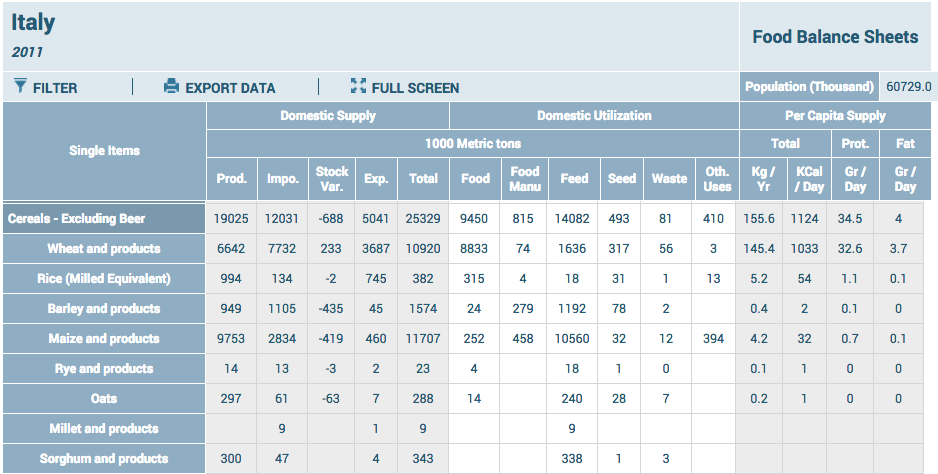
\includegraphics[width=\maxwidth]{figure/fbs_italy_2011.png} 
}
\caption[First lines of the FBS for Italy in 2011.]{First lines of the FBS for Italy in 2011.
\label{tab:fbs_italy_2011}}

\end{figure}
\end{knitrout}

\subsection{Balancing equation}
The term "balancing table" refers to the attempt to balance accounts 
in each country for each commodity between its supply (Production, 
Imports, Stock Changes and Exports) and its uses (Food, Food Manufacturing, 
Feed, Seed, Waste,  and Other Uses).\\
For each commodity $i$ in a given country $c$ at time $t$ the Total Supply 
(TU) and the Total Domestic Utilization (TU) are described as following: 

\begin{align}
	{\text TS}_{c,t,i} &= {\text Production}_{c,t,i} + {\text Imports}_{c,t,i} 
	+ {\text StockVar}_{c,t,i} - {\text Exports}_{c,t,i}\\
	{\text TU}_{c,t,i} & = {\text Food}_{c,t,i} + {\text FoodManu}_{c,t,i} 
	+ {\text Feed}_{c,t,i} + {\text Seed}_{c,t,i} + {\text Waste}_{c,t,i} 
	+ {\text OtherUses}_{c,t,i}
\end{align}

Where with ${\text StockVar}_{c,t,i}$ we consider the difference between 
the level of stock at time $t$ and time $t-1$. In order to have a "balanced" 
or "closed" FBS the following balance identity needs to hold:

\begin{equation}\label{eq}
{\text TS}_{c,t,i} = {\text TU}_{c,t,i} \quad\quad \forall i
\end{equation}

The identity \ref{eq} is often not respected, due to the uncertainty of data, 
as explained in the previous section. Mahjoubi and Prakash (2012) and 
FAO (2014)

\subsection{Methods for  estimate TS and TU}
Apart from Production and trade (Imports and Exports), which are collected 
through questionnaires, all  other elements of the FBS are usually estimated 
and official data are available only for very few developed countries (Mahjoubi 
and Prakash, 2012, and FAO, 2014).

\subsubsection{Production and trade}
Due to these elements' reliability, these elements drive the FBS production system. 
Consequently, data collection efforts, especially in the Production domain, that 
rely on questionnaire response, remain key. The information that FBS supplies 
ultimately can only be as good as the core underlying data, and concerted action 
is required to improve data inflows.\\

More can be said about Production imputation, reference Michael's paper.

\subsubsection{Food}
This term represents the total supply of all agricultural and derived products 
available for human consumption. Food available can be reported in terms of 
primary product equivalent such as wheat and milk or in the form that the products 
may actually be consumed, such as bread and cheese. This number is typically 
the residual of the balance sheet. However, due to uncertainty surrounding many 
other elements of the balance and because of weak methods and outdated 
parameters, food is not the only residual element. In order to have an accurate 
estimate for food measurement  a methodological framework for incorporating 
information from other existing statistical sources of information, i.e. Nationally 
representative Household Survey (NHS) is under development. \\

Jim work. Reference as soon as available.

\subsubsection{Food Processing}
This term, also known as Food Manufacturing, is the amount of a commodity 
processed for food purposes and for which separate entries are provided in the 
FBSs either in the same commodity tree or in another food commodity. This 
helps to maintain the concept of accounting for all foods (once and only once) 
and maintains the links in the various levels of the balance sheets.

\subsubsection{Feed}
This term represents the quantity of the commodity available for feeding to 
livestock and poultry during the year. Less than 15\% of the countries respond 
to FAO�s feed questionnaire and most of them are developed countries. For the 
rest of the world, a new method was developed. It is divided in two steps: 
\begin{itemize}
\item[i] determine feed requirements for metabolizable energy and protein 
\item[ii] determine allocation of compound/concentrate feedstuffs to match 
requirements. 
\end{itemize}

See FAO (2014) for more details, and reference Onno work.

\subsubsection{Seed}
Among the different categories of utilization, Seed use is one of the few categories 
which can be modeled a priori according to a deterministic rule, animal feed is 
possibly another. Seeding rates, and ultimately the demand for seed, can be modeled 
as a function of target plant density, establishment percentage, and seed weight. 
Multiplied by area planted, seed use can then be derived. However, with the rise 
in high-precision commercial farming, many farmers are choosing to use certified 
seed, purchased from specialized seed farmers. This trend requires the need to 
capture commercial seed production quantities.\\

Reference Josh work. 

\subsubsection{Waste}
This term is the amount of the commodity lost through wastage during the year 
at all stages between farms and the household level in handling, storage and transport, 
but not including waste in the edible and inedible part of the commodity which occurs 
after the commodity has entered the household. The quantities lost during processing 
are also not included under this element because they are implicitly considered in applying 
the underlying extraction rate. Waste data have been reviewed for some 140 developing 
countries. It can be seen that the coefficients developed to calculate waste in FAOSTAT 
(waste is calculated as a percentage of total supply) have been constant for many years. 
Moreover, the review shows inconsistencies in the waste parameters among countries, 
and commodities within countries.\\

Reference Klaus work.

\subsubsection{Other Utilization}
This term is a miscellaneous category to account for all other uses not identified 
elsewhere (e.g. the use of maize to produce ethanol). This category also includes 
consumption by those who are not accounted in the country�s population 
(e. g., tourists).\\

Reference Jim work on tourism. 

\subsubsection{Stock Changes}
Limited information exists on opening or closing stocks for many commodities in 
many countries, making stocks estimation complicated and imprecise. As a result, 
stock changes are often calculated to smooth supply and utilization. In practice, 
they are used as a balancing factor and they may, in part, be calculated residually 
by first estimating food available for consumption. As the item is partially and 
residually derived it then reflects not only stock changes but also other statistical 
errors in the food balance equation.

\section{An alternative approach to balance FBSs}
\subsection{Problem formulation}
A generale FBS looks like the following


\begin{table}[h!]
  \label{tab:example}
  \caption{Scheme of the FBS}
  \begin{center}
    \begin{tabular}{|c||c|c|c|c|c|c||c|}
      \hline
       & $L_1$&$L_2$&$\dots$&$L_j$&$\dots$&$L_s$&$Tot Rows$\\
       \hline\hline
       $C_1$ & $x_{11}$&$x_{12}$&$\dots$&$x_{1j}$&$\dots$&$x_{1s}$&$R_1$\\
       \hline
        $C_2$ & $x_{21}$&$x_{22}$&$\dots$&$x_{2j}$&$\dots$&$x_{2s}$&$R_2$\\
        \hline
        $\dots$ & $\dots$&$\dots$&$\dots$&$\dots$&$\dots$&$\dots$&$\dots$\\
        \hline
        $C_i$ & $x_{i1}$&$x_{i2}$&$\dots$&$x_{ij}$&$\dots$&$x_{is}$&$R_i$\\
        \hline
        $\dots$ & $\dots$&$\dots$&$\dots$&$\dots$&$\dots$&$\dots$&$\dots$\\
        \hline
        $C_r$ & $x_{r1}$&$x_{r2}$&$\dots$&$x_{rj}$&$\dots$&$x_{rs}$&$R_r$\\
        \hline\hline
        $Tot Cols$ & $T_{1}$&$T_{2}$&$\dots$&$T_{j}$&$\dots$&$T_{s}$&Tot\\
      \hline
    \end{tabular}
  \end{center}  
\end{table}

Each row $C_i$ represents a commodity and each column $L_j$ represents a level, both supply or utilization.  The table satisfies the following identities:

\begin{align}
	R_i &= \sum_{j=1}^{s}x_{ij}\\
	T_j & = \sum_{i=1}^{r}x_{ij}\\
	Tot & = \sum_{i=1}^{r} R_i = \sum_{j=1}^{s} T_j = \sum_{i=1}^{r}\sum_{j=1}^{s}x_{ij}
\end{align}	

First of all, we assume that for each commodity $C_i$, its total row  $R_i$ is fixed. 
This means that we rearrange the balancing identity shown in \ref{eq} placing to 
the left of the equation the terms that come from official sources, hereafter called 
consolidated terms, and to right those coming from unofficial sources. In our 
example, Production is the only consolidated term. Then, the balancing identity
 \ref{eq} can be rewritten in the following way:

\begin{align}
	{\text Production}_{c,t,i} = & - {\text Imports}_{c,t,i} - {\text StockVar}_{c,t,i} + 
	{\text Exports}_{c,t,i} \\
	 & + {\text Food}_{c,t,i} + {\text FoodManu}_{c,t,i} 
	+ {\text Feed}_{c,t,i} + {\text Seed}_{c,t,i} + {\text Waste}_{c,t,i} 
	+ {\text OtherUses}_{c,t,i}
\end{align}	

where ${\text StockVar}_{c,t,i} = {\text Stock}_{c,t,i} - {\text Stock}_{c,t-1,i}$. Then the FBS assumes the form of the following table:

\begin{table}[h!]
  \label{tab:fbstab}
  \caption{Scheme of the FBS}
  \begin{center}
    \begin{tabular}{|c||c|c|c|c|c|c|c|c|c||c|}
      \hline
       & Imps&StockV&Exps&Food&FoodM&Feed&Seed&Waste&Other&Production\\
       \hline\hline
       $C_1$ & $x_{11}$ & $x_{12}$ & $x_{13}$ & $x_{14}$ & $x_{15}$ & $x_{16}$ & $x_{17}$ & $x_{18}$ & $x_{19}$ & $R_{1}$\\
       \hline
       $C_2$ & $x_{21}$ & $x_{22}$ & $x_{23}$ & $x_{24}$ & $x_{25}$ & $x_{26}$ & $x_{27}$ & $x_{28}$ & $x_{29}$ & $R_{2}$\\
       \hline
        $\dots$ & $\dots$ & $\dots$ & $\dots$ & $\dots$ & $\dots$ & $\dots$ & $\dots$ & $\dots$ & $\dots$ & $\dots$\\
        \hline
       $C_i$ & $x_{i1}$ & $x_{i2}$ & $x_{i3}$ & $x_{i4}$ & $x_{i5}$ & $x_{i6}$ & $x_{i7}$ & $x_{i8}$ & $x_{i9}$ & $R_{i}$\\
       \hline
        $\dots$ & $\dots$ & $\dots$ & $\dots$ & $\dots$ & $\dots$ & $\dots$ & $\dots$ & $\dots$ & $\dots$ & $\dots$\\
        \hline
       $C_r$ & $x_{r1}$ & $x_{r2}$ & $x_{r3}$ & $x_{r4}$ & $x_{r5}$ & $x_{r6}$ & $x_{r7}$ & $x_{r8}$ & $x_{r9}$ & $R_{r}$\\
        \hline\hline
        $Tot Cols$ & $T_{1}$&$T_{2}$&$T_{3}$&$T_{4}$&$T_{5}$&$T_{6}$&$T_{7}$&$T_{8}$&$T_{9}$&Tot\\
      \hline
    \end{tabular}
  \end{center}  
\end{table}

In the same way, if we believe that the consolidates terms are more than one, i.e. Production and trade (Imports and Exports), the balancing identity can be rewritten as follows:

\begin{align}
	{\text Production}_{c,t,i} + {\text Imports}_{c,t,i} - {\text Exports}_{c,t,i} & =  {\text StockVar}_{c,t,i} + {\text Food}_{c,t,i}\\
	 & + {\text FoodManu}_{c,t,i} + {\text Feed}_{c,t,i} + {\text Seed}_{c,t,i} \\
	 & + {\text Waste}_{c,t,i} + {\text OtherUses}_{c,t,i}
\end{align}	


In this way, we consider data from official sources as highly accurate and reliable data, 
while those from non-official sources prone to potential measurement errors. 
The latter are often estimated or adjusted with a certain degree of error that depends 
on differing concepts, definitions, and methodologies involved in data gathering and 
generation among countries (Jacobs and Sumner, 2002). For these reasons, the 
consolidated terms may change from country to country, and from year to year. \\
Then, we assume that all ammounts  $x_{ij}$ are measured with an additive error:
\begin{equation}
y_{ij}= x_{ij}+e_{ij} \quad\quad    \forall i,j
\end{equation}

where $y_{ij}$ represents the true commodity value and $e_{ij}$ is the difference 
between the measured value and its true value.\\
As discussed in Robinson et al. (2000), the classical assumptions made in 
regression analysis ${\text Cov}(x_{ij},e_{ij})=0$ with $e_{ij}\sim  \mathscr{N} (0,\sigma^2 )~~\forall i,j$ are extremely constraining when little is known about the error of structure and data are scarse.
Even if a normal distribution can be attributed to $e_{ij}$, the assumption of zero mean 
seems not realistic in our case.\\
To take into account the measurement error of the individual cells ($x_{ij}$), we assume 
for these values a Normal truncated distribution:
\begin{equation}
x_{ij} \sim TN (\mu_{ij},\sigma_{ij}^2)
\end{equation}

%The values of each $\mu_{ij}$ are the results of the estimation methods used for the elements of the TS and TU (see Subsection 2.2). Instead, the standard deviation reflects the degree of uncertainty that the researcher has on estimaed value �_ij. Then, it is very important for the researcher have a good understanding of the data, to know then how from which country they are they was generated or collected.
%Note that how this allows us to integrate the inaccurate information, represented by the estimated mean with a measure or how much each value is trusted and with expert knowledge which informs us the bounds of the cell value. The shape of the distribution will change depending on the prior information the researcher has for that particular commodity C in that particular level L. Those levels, which have measured with more accuracy, will have a narrower distribution, otherwise the researcher will use a more vague and uniform-like prior. Because a FBS often contains values that are null with certainty, i.e., quantities of processed seed use are not measured in the amount of eggs, we allow some cells x_ij to be constrained to be null. We call those elements structural zeros. 
%Also, beacuse the column totals T_j are not fixed, the range of the possible outcomes for T_j is given by experts as the interval  (t_(j,min),t_(j,max)).  Since the only strong constraint is the one on the row totals, we need to choose a strategy to 


\section*{Acknowledgement}
This work is supervised by Adam Prakash with assistance from Josef
Schumidhuber, Onno Hoffmeister, Salar Tayyib  whom were crucial in 
the development of the methodology. The author would also like to thank 
the team members which participated in the previous discussions providing 
valuable feedbacks.

\section*{Annex 1: Supplementary Resources}

The data, source code and documentation can all be found and
downloaded from \url{https://github.com/marcogarieri/conSTable/tree/develop}, the
package can also be installed by following the instruction. 

\FloatBarrier
\section*{Annex 2: Pseudo Codes}
     

\begin{algorithm}[H]
  \SetAlgoLined
  \KwData{Production (element code = 51) and Harvested area (element
    code = 31) data}

  \KwResult{Imputation}
  
  \BlankLine
  Missing values are denoted $\emptyset$\;

  \BlankLine
  Initialization\;
  \Begin{
      \If{$A_t = 0 \land P_t \ne 0$}{
        $A_t \leftarrow \emptyset$\;
      }
      \If{$P_t = 0 \land A_t \ne 0$}{
        $P_t \leftarrow \emptyset$\;
      }
  }  
    
  \BlankLine  
  Start imputation\;
  \Begin{
      \ForAll{commodities}{
        
        (1) Compute the implied yield\;
        \Indp\Indp\Indp 
        $Y_{i,t} \leftarrow P_{i,t}/A_{i,t}$\;
        \Indm\Indm\Indm
                
        (2) Impute the missing yield with the yield algorithm
        \; \Indp\Indp\Indp
        
        \Indm\Indm\Indm        
        
        \ForAll{imputed yield $\hat{Y}_{i, t}$}{
          \If{$A_t = \emptyset \land P_t \ne \emptyset$}{
            $\hat{A}_{i, t} \leftarrow P_{i, t}/\hat{Y}_{i, t}$\;
          }
          \If{$P_t = \emptyset \land A_t \ne \emptyset$}{
            $\hat{P}_{i, t} \leftarrow A_{i, t} \times \hat{Y}_{i, t}$\;
          }
        }
        
        (4) Impute production ($P_{i, t}$) with ensemble\;
        
        \ForAll{imputed production $\hat{P}_{i, t}$}{ \If{$\hat{Y}_{i, t}
            \ne \emptyset$}{ $\hat{A}_{i, t} \leftarrow \hat{P}_{i, t}/
            \hat{Y}_{i, t}$\; } } } }
  \caption{Imputation Procedure - function
    \emph{swsProductionImputation}}
\end{algorithm}

  
  
\begin{thebibliography}{11}
\bibitem{dougbates2010}
  Douglas M. Bates,
  \emph{lme4: Mixed-effects modelling with R},
  2010.
  
\bibitem{impWorkingPaper2011}
  Data Collection, Workflows and Methodology (DCWM) team,
  \emph{Imputation and Validation Methodologies for the FAOSTAT Production Domain},
  Economics and Social Statistics Division,
  2011.
  
\bibitem{lairdWare1982}
  Nan M. Laird, James H. Ware,
  \emph{Random-Effects Models for Longitudinal Data},
  Biometrics Volume 38, 963-974,
  1982.
  
\bibitem{rCore}
  R Core Team,
  \emph{A language and environment for statistical computing.},
  R Foundation for Statistical Computing, Vienna, Austria,
  ISBN 3-900051-07-0, URL http://www.R-project.org/,
  2013.
  
\bibitem{nlme}
  Jose Pinheiro, Douglas Bates, Saikat DebRoy, Deepayan Sarkar and the
  R Development Core Team,
  \emph{nlme: Linear and Nonlinear Mixed Effects Models.} ,
  R package version 3.1-108,
  2013.

\bibitem{lme4}
  Douglas Bates, Martin Maechler, Ben Bolker and Steven Walker,
  \emph{lme4: Linear mixed-effects models using Eigen and S4.} 
  R package version 1.0-4. http://CRAN.R-project.org/package=lme4,
  2013.
 
\bibitem{rubin1976}
  Donald B. Rubin,
  \emph{Inference and Missing Data},
  Biometrika, Volume 63, Issue 3, 581-592,
  1976.
  
\bibitem{unido2012}
  Valentin Todorov, Matthias Templ,
  \emph{R in the Statistical Office: Part II},
  2012.
  
\bibitem{laird_ware1982}
  Nam M. Laird, James H. Ware,
  \emph{Random-Effects Models for Longitudinal Data},
  Biometrics, Volume 38, Number 4, pp.963-974,
  1982.

\bibitem{dempster_laird_rubin1977}
  A. P. Dempster, Nam M. Laird, D. B. Rubin,
  \emph{Maximum Likelihood from Incomplete Data via the EM Algorithm},
  Journal of Royal Statistical Society. Series B (Methodological), Volume 39, Number 1, pp1-38,
  1977.
  
\bibitem{lai_huang_lee2012}
  Randy C. S. Lai, Hsin-Cheng Huang, Thomase C. M. Lee,
  \emph{Fixed and random effects selection in nonparametric additive mixed models},
  Electronic Journal of Statistics, Volume 6, pp810-842,
  2012.
\end{thebibliography}
  




\end{document}
Status API Training Shop Blog About
� 2015 GitHub, Inc. Terms Privacy Security Contact
%